
\documentclass[ignorenonframetext, professionalfonts, hyperref={pdftex, unicode}]{beamer}

\usetheme{Copenhagen}
\usecolortheme{wolverine}

\usepackage[orientation=landscape, size=custom, width=16, height=9.75, scale=0.5]{beamerposter}	

%Packages to be included

\usepackage{textcomp}

\usepackage[russian]{babel}
\usepackage[utf8]{inputenc}
\usepackage[T1]{fontenc}

\usepackage{beamerthemesplit}

\usepackage{ulem}

\usepackage{verbatim}

\usepackage{ucs}
\usepackage{listings}
\lstloadlanguages{C, make, bash}

\lstset{escapechar=`,
	extendedchars=false,
	language=C, 
	tabsize=2, 
	columns=fullflexible, 
%	basicstyle=\scriptsize,
	keywordstyle=\color{blue}, 
	commentstyle=\itshape\color{brown},
%	identifierstyle=\ttfamily, 
	stringstyle=\mdseries\color{green}, 
	showstringspaces=false, 
	numbers=left, 
	numberstyle=\tiny, 
	breaklines=true, 
	inputencoding=utf8x,
	keepspaces=true,
	morekeywords={u\_short, u\_char, u\_long, in\_addr}
	}

\definecolor{darkgreen}{cmyk}{0.7, 0, 1, 0.5}

\lstdefinelanguage{diff}
{
    morekeywords={+, -},
    sensitive=false,
    morecomment=[l]{//},
    morecomment=[s]{/*}{*/},
    morecomment=[l][\color{darkgreen}]{+},
    morecomment=[l][\color{red}]{-},
    morestring=[b]",
}



%%%%%%%%%%%%%%%%%%%%%%%%%%%%%%%%%%%%%%%%%%%%%%%%%
%%%%%%%%%% PDF meta data inserted here %%%%%%%%%%
%%%%%%%%%%%%%%%%%%%%%%%%%%%%%%%%%%%%%%%%%%%%%%%%%
\hypersetup{
	pdftitle={Введение в GNU/Linux},
	pdfauthor={Epam/LLPD}
}





%%%%%% Beamer Theme %%%%%%%%%%%%%

	
\title{Введение в GNU/Linux}
\author{Epam/LLPD}



%%%%%%%%%%%%%%%%%%%%%%%%%%%%%%%%%%%%%%%%%%%%%%%%%
%%%%%%%%%% Begin Document  %%%%%%%%%%%%%%%%%%%%%%
%%%%%%%%%%%%%%%%%%%%%%%%%%%%%%%%%%%%%%%%%%%%%%%%%




\begin{document}

\frame{
	\frametitle{Дисковая подсистема}
	\titlepage
	\vspace{-0.5cm}
	\begin{center}
	%\frontpagelogo
	\end{center}
}
\frame{
	\tableofcontents
%	[hideallsubsections]
}

%\section{}

\begin{frame}{Дисковая подсистема}

	\begin{block}{Блочное устройство}
		Вид файла устройств в UNIX/Linux-системах,  обеспечивающий интерфейс к устройству,
		реальному или виртуальному, в виде файла в файловой системе.
	\end{block}

	\begin{block}{Файловая система}
		Файловая система определяет формат содержимого и способ физического хранения информации,  
		которую принято группировать в виде файлов. 
		Конкретная файловая система определяет размер имени файла (директории),  
		максимальный возможный размер файла и раздела,  набор атрибутов файла.

		Распространенные для ОС Linux: ext2, ext4, xfs, reiserfs, vfat.
	\end{block}
\end{frame}

\begin{frame}{Примеры блочных устройств}

	\begin{itemize}
		\item {\tt /dev/{\bf s}d*}
		\item {\tt /dev/{\bf h}d*}
		\item {\tt /dev/ram*}
		\item {\tt /dev/loop*}
	\end{itemize}

	\begin{block}{Практическое задание:}
		\begin{enumerate}
			\item Посмотреть список вышеперечисленных устройств
			\item Посмотреть информацию об устройствах {\tt loop0, ram, sda}\\
				Hint: {\tt fdisk -l <device>}
		\end{enumerate}
	\end{block}
\end{frame}

\begin{frame}{Структура диска}
	\begin{columns}
		\column{0.6\textwidth}
		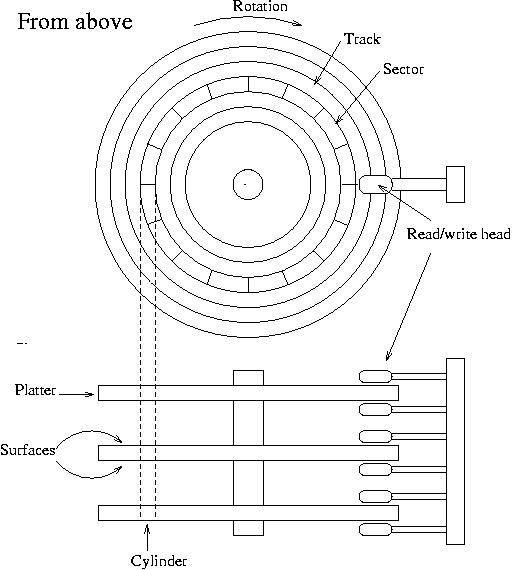
\includegraphics[height=0.8\textheight]{04-hd-schematic.png}
		\column{0.4\textwidth}
		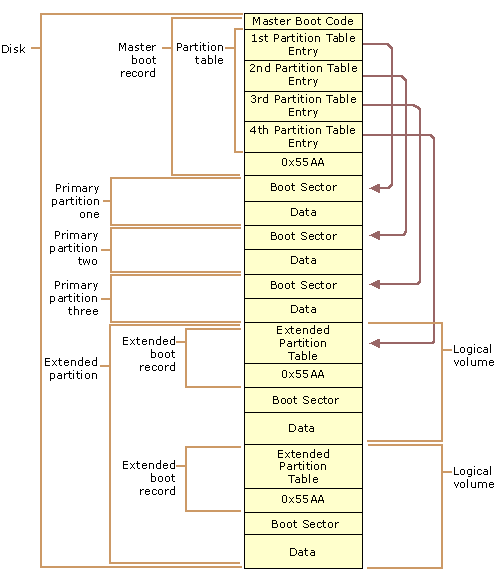
\includegraphics[height=0.8\textheight]{04-disk-structure.png}
	\end{columns}
\end{frame}

\begin{frame}{Отображение блочных устройств}


	\begin{block}{Device Mapper}
			{\tt /dev/mapper/*}\\
			device-mapper -- служит общим фреймворком для отображения одного блочного устройства на другое.

			Примеры: RAID, LVM, шифрованные диски и т.д.
	\end{block}

\end{frame}



\begin{frame}{Полезные утилиты}
	\begin{columns}
		\column{0.25\textwidth}
		\begin{itemize}
			\item {\tt fdisk}
			\item {\tt parted}
			\item {\tt kpartx}
		\end{itemize}
		\column{0.25\textwidth}
		\begin{itemize}
			\item {\tt dd}
			\item {\tt losetup}
		\end{itemize}
		\column{0.25\textwidth}
		\begin{itemize}
			\item {\tt mkfs}
			\item {\tt fsck}
		\end{itemize}
		\column{0.25\textwidth}
		\begin{itemize}
			\item {\tt mount}
			\item {\tt umount}
			\item {\tt df}
		\end{itemize}
	\end{columns}

	\bigskip
	Понадобятся для упражнений:
	\begin{itemize}
			\item[*] {\tt chroot}
			\item[*] {\tt kvm}
	\end{itemize}
\end{frame}


\begin{frame}{Практика: отображение файла на loop-устройство}
	\begin{enumerate}
		\item Создать пустой файл размером 100MB: \\
			dd if=/dev/zero of=test bs=1M count=100
			\pause
		\item Найти неиспользуемое loop-устройство и отобразить на него файл:\\
			losetup -f \\
			losetup loop0 test
			\pause
		\item Посмотреть структуру loop-устройства, создать разделы и посмотреть результаты:\\
			fdisk -l /dev/loop0 \\
			fdisk /dev/loop0 \\
			fdisk -l /dev/loop0
			\pause
		\item Дать команду ядру перечитать разделы и создать устройства для разделов:\\
			ls -l /dev/mapper/* \\
			kpartx -a /dev/loop0 \\
			ls -l /dev/mapper/* \\
	\end{enumerate}
\end{frame}

\begin{frame}{Практика: создание файловой системы}
	\begin{enumerate}
		\item Форматируем файловую систему на устройстве: \\
			mkfs.ext2 /dev/mapper/loop0p1
			\pause
		\item и монтируем:\\
			mkdir -p /mnt/fs\\
			mount\\
			mount /dev/mapper/loop0p1 /mnt/fs\\
			mount\\
			df
			\pause
	\end{enumerate}
\end{frame}


\begin{frame}{Практика: чистимся}
	\begin{enumerate}
		\item Найти смонтированные разделы и отмонтировать их: \\
			mount \\
			umount /dev/mapper/loop0p1
			\pause
		\item Найти используемые loop-устройства\\
			losetup -a \\
			\pause
		\item Корректно удалить устройства для разделов:\\
			ls -l /dev/mapper/* \\
			kpartx -d /dev/loop0 \\
			ls -l /dev/mapper/* \\
			\pause
		\item Удалить отображение файла на loop-устройство: \\
			losetup -d /dev/loop0
	\end{enumerate}
\end{frame}

\end{document}
